\subsection{The method of characteristics}
\label{m:sec:moc}

Every generating-function equation met above is first order: \cref{m:eq:bdpde} for
the birth--death process, and the bivariate equations of
\cref{m:app:absorption} for the absorption models. That is not a coincidence but a
consequence of linear rates, and it is worth exploiting, because first-order
equations have a general solution method. This subsection presents it.

\subsubsection{The idea}
\label{m:sec:mocidea}

A first-order partial differential equation says that a certain directional
derivative of the unknown function is prescribed. If one can find the curves along
which that direction points --- the \emph{characteristics} --- then along each such
curve the equation collapses to an ordinary differential equation, which can be
solved. The solution is then transported along the curve back to a surface where
the initial data are known.

Concretely, suppose $G$ satisfies
\begin{equation}
\label{m:eq:genericfirstorder}
\pddt{G} = a(x,y)\pdd{G}{x} + b(x,y)\pdd{G}{y},
\qquad
G(x,y,0) = G_0(x,y) .
\end{equation}
Reparametrise the independent variables as $(x,y,t)\to(\sigma,\eta,\tau)$, where
$\sigma$ and $\eta$ label a characteristic curve and $\tau$ runs along it. Along
such a curve $G$ is a function of $\tau$ alone, so the chain rule gives
\begin{equation}
\label{m:eq:chainrule}
\dda{G}{\tau}
= \pddt{G}\dda{t}{\tau} + \pdd{G}{x}\dda{x}{\tau} + \pdd{G}{y}\dda{y}{\tau} .
\end{equation}
Comparing this with \cref{m:eq:genericfirstorder} rewritten as
$0 = -\partial_tG + a\,\partial_xG + b\,\partial_yG$ and matching the coefficient of
each partial derivative gives the \emph{characteristic system}
\begin{equation}
\label{m:eq:genericcharacteristics}
\dda{G}{\tau} = 0,
\qquad
\dda{t}{\tau} = -1,
\qquad
\dda{x}{\tau} = a(x,y),
\qquad
\dda{y}{\tau} = b(x,y) .
\end{equation}
Four ordinary differential equations have replaced one partial differential
equation. The first says that $G$ is constant along characteristics, so $G$ depends
only on the labels $(\sigma,\eta)$; the second says the parameter runs backwards in
time, which is what allows the initial surface to be reached from any $(x,y,t)$; the
last two are the curves themselves.

The parametrisation is fixed by anchoring the labels to the initial surface,
\begin{equation}
\label{m:eq:ICpar}
x(\sigma,\eta,0)=\sigma,
\qquad
y(\sigma,\eta,0)=\eta,
\qquad
t(\sigma,\eta,0)=0 ,
\end{equation}
so that $G(\sigma,\eta,\tau)=G_0(\sigma,\eta)$. The whole problem then reduces to a
change of variables: express $\sigma$ and $\eta$ in terms of $(x,y,t)$ by
integrating the characteristic equations and substitute. That final substitution is
where the work lies.

\Cref{m:fig:characteristics} shows the geometry for the $x$-equation of the example
that follows.

\begin{figure}[ht]
\centering
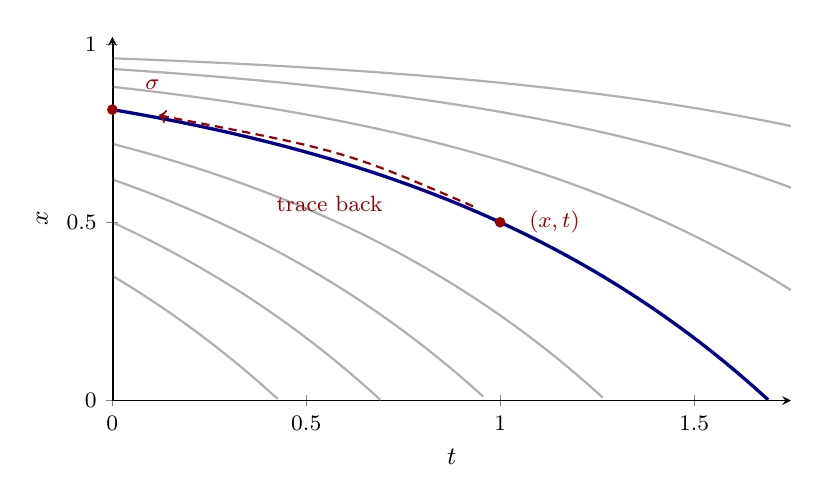
\begin{tikzpicture}
\begin{axis}[
  width=10.2cm, height=6.2cm,
  axis lines=left,
  xlabel={$t$}, ylabel={$x$},
  xmin=0, xmax=1.75, ymin=0, ymax=1.02,
  xtick={0,0.5,1,1.5}, ytick={0,0.5,1},
  tick label style={font=\footnotesize},
  label style={font=\small},
  clip=true,
  restrict y to domain=0:1.05,
  samples=120,
]
% the characteristic family x(t) = 1-(1-sigma)e^{mu t}, mu = 1
\foreach \s in {0.35,0.5,0.62,0.72,0.88,0.93,0.96} {
  \addplot[gray!62, thick, domain=0:1.75] {1-(1-\s)*exp(x)};
}
% the highlighted characteristic through (t,x) = (1, 0.5): sigma = 1-0.5e^{-1}
\addplot[blue!55!black, very thick, domain=0:1.75] {1-(0.5/2.718281828)*exp(x)};
% initial surface
\draw[black, very thick] (axis cs:0,0) -- (axis cs:0,1.0);
% the evaluation point and its foot
\addplot[only marks, mark=*, mark size=1.7pt, red!60!black]
      coordinates {(1,0.5)};
\addplot[only marks, mark=*, mark size=1.7pt, red!60!black]
      coordinates {(0,0.8161)};
\node[font=\footnotesize, anchor=west, red!60!black] at (axis cs:1.05,0.5) {$(x,t)$};
\node[font=\footnotesize, anchor=south west, red!60!black]
      at (axis cs:0.06,0.845) {$\sigma$};
% back-arrow along the highlighted curve
\draw[->, red!60!black, thick, densely dashed]
      (axis cs:0.93,0.545) .. controls (axis cs:0.6,0.70) .. (axis cs:0.12,0.80);
\node[font=\footnotesize, anchor=north, red!60!black]
      at (axis cs:0.56,0.60) {trace back};
\end{axis}
\end{tikzpicture}
\caption{Characteristics of the $x$-equation \cref{m:eq:ch13},
$\dd x/\dd\tau=\mu(1-x)$ with $\tau=-t$, drawn for $\mu=1$. Each grey curve is one
characteristic, $x(t)=1-(1-\sigma)\ee^{\mu t}$, labelled by the point $\sigma$ at
which it meets the initial surface $t=0$, drawn as the heavy vertical line;
together they foliate the domain, and
exactly one passes through any given $(x,t)$. Since $G$ is constant along
characteristics, its value at a point is its value at the foot of that point's
curve --- so solving the equation amounts to running the curve backwards from
$(x,t)$ to $t=0$ and reading off $\sigma$, here $\sigma=1-(1-x)\ee^{-\mu t}$. The
full problem is three-variate; this is its projection onto the $(x,t)$ plane, which
is where the cascade starts, because \cref{m:eq:ch13} does not involve $y$.}
\label{m:fig:characteristics}
\end{figure}

\subsubsection{A worked example: absorption--death}
\label{m:sec:mocworked}

The example is chosen so that the answer can be checked. Consider a single
compartment that takes in particles from a surrounding medium, in which a resident
particle may then die; \cref{m:fig:compartment} sets out the geometry, which is
common to every absorption model in this thesis. Let $X_t$ count particles inside
the compartment and $Y_t$ those outside, and let the events be
\begin{align*}
\pr{\Delta X=1,\ \Delta Y=-1\mid Y_t=j} &= j\alpha\,\Delta t, &&\text{(absorption)}\\
\pr{\Delta X=-1,\ \Delta Y=0\mid X_t=i} &= i\mu\,\Delta t, &&\text{(death)}\\
\pr{\Delta X=0,\ \Delta Y=0\mid X_t=i,\ Y_t=j} &= 1-(j\alpha+i\mu)\Delta t, &&\text{(no event)}
\end{align*}
with terms of $o(\Delta t)$ suppressed. Each exterior particle is independently
taken up at rate $\alpha$ and each interior one dies at rate $\mu$. The initial
condition is $X_0=0$, $Y_0=N$.

\begin{figure}[ht]
\centering
\begin{tikzpicture}[
  >={Stealth[length=2.2mm]},
  every path/.style={thick},
  pt/.style={circle, fill=black!62, inner sep=0pt, minimum size=3.1pt},
  ptin/.style={circle, fill=blue!55!black, inner sep=0pt, minimum size=3.1pt},
  lb/.style={font=\footnotesize},
  note/.style={font=\footnotesize\itshape, text=black!65}
]
% ---- exterior medium ------------------------------------------------------
\draw[rounded corners=5pt, draw=black!35, fill=black!4]
      (0,0) rectangle (10.6,4.5);
\node[note, anchor=north west] at (0.18,4.36) {exterior medium};
\node[lb, anchor=north west] at (0.18,3.92) {$Y_t$ particles};
\foreach \x/\y in {0.8/1.15, 1.45/2.35, 0.95/3.05, 2.05/0.72, 2.3/1.75,
                   1.7/3.35, 2.85/2.6, 3.35/1.25, 2.6/3.55, 3.75/2.95,
                   3.95/1.15, 3.05/0.55, 4.35/3.4, 1.15/1.95}
  \node[pt] at (\x,\y) {};

% ---- compartment ----------------------------------------------------------
\draw[rounded corners=5pt, draw=black!75, very thick, fill=white]
      (6.0,0.75) rectangle (10.0,3.75);
\node[note, anchor=north west] at (6.18,3.62) {compartment};
\node[lb, anchor=north west] at (6.18,3.20) {$X_t$ particles};
\foreach \x/\y in {6.8/1.35, 7.5/2.05, 8.3/1.6, 7.9/2.6, 9.0/2.25, 8.6/1.1}
  \node[ptin] at (\x,\y) {};

% ---- absorption -----------------------------------------------------------
\draw[->, draw=blue!45!black, line width=1pt] (4.95,2.25) -- (5.85,2.25);
\node[lb, anchor=south, text=blue!45!black] at (5.40,2.36) {$\alpha$};
\node[note, anchor=north east] at (5.88,2.14) {absorption};

% ---- birth (interior) -----------------------------------------------------
\draw[->, draw=black!75] (9.32,2.55) arc (-60:205:0.40);
\node[lb, anchor=west] at (9.42,3.05) {$\lambda$};

% ---- death (interior) -----------------------------------------------------
\node[font=\small] (void) at (8.15,0.12) {$\varnothing$};
\draw[->, draw=black!75] (8.15,0.95) -- (void);
\node[lb, anchor=west] at (8.28,0.52) {$\mu$};
\end{tikzpicture}
\caption{The single-compartment absorption models. Particles begin in the exterior
medium and are taken up one at a time, each independently at rate $\alpha$, so the
absorption channel carries total rate $Y_t\alpha$; once inside, a particle dies at
rate $\mu$ and, in the fullest version of the model, divides at rate $\lambda$.
Only the three transitions drawn here occur, and each is proportional to the count
in the compartment it acts on. Note that nothing returns from the compartment to
the medium, which is why the exterior count is unaffected by the interior
dynamics.}
\label{m:fig:compartment}
\end{figure}

The forward equations \cref{m:eq:master} read
\begin{equation}
\label{m:eq:FK2}
\ddt{p_{i,j}} = \alpha(j+1)p_{i-1,j+1} + \mu(i+1)p_{i+1,j} - (\alpha j+\mu i)p_{i,j},
\end{equation}
and the construction of \cref{m:sec:backward}, applied to the bivariate generating
function \cref{m:eq:pgfbivariate}, converts them into
\begin{equation}
\label{m:eq:PDE2}
\pddt{G} = \mu(1-x)\pdd{G}{x} + \alpha(x-y)\pdd{G}{y},
\qquad
G(x,y,0) = y^N .
\end{equation}

Without births the particles never interact, so
each of the $N$ of them is independently in one of three states at time $t$ ---
outside, inside, or dead --- and the generating function is a power of the
single-particle one. The single-particle state probabilities satisfy
$\dd p_{0,1}/\dd t = -\alpha p_{0,1}$ and
$\dd p_{1,0}/\dd t = \alpha p_{0,1}-\mu p_{1,0}$, giving
\begin{equation}
\label{m:eq:absdeathstates}
p_{0,1}(t) = \ee^{-\alpha t},
\qquad
p_{1,0}(t) = \frac{\alpha}{\mu-\alpha}\lrb{\ee^{-\alpha t}-\ee^{-\mu t}},
\qquad
p_{0,0}(t) = 1-p_{0,1}(t)-p_{1,0}(t),
\end{equation}
plotted in \cref{m:fig:abs2}, and hence
\begin{equation}
\label{m:eq:Gabsdeath}
G(x,y,t) = \Bigl(
1-\tfrac{\mu}{\mu-\alpha}\ee^{-\alpha t} + \tfrac{\alpha}{\mu-\alpha}\ee^{-\mu t}
+ \tfrac{\alpha}{\mu-\alpha}\bigl(\ee^{-\alpha t}-\ee^{-\mu t}\bigr)x
+ \ee^{-\alpha t}y\Bigr)^{N} .
\end{equation}
So \cref{m:eq:PDE2} can be solved by characteristics with the answer known in
advance.\footnote{I am grateful to Benjamin Sharp for the advice on applying the
method of characteristics to three-variate problems that unlocked this
calculation.}

\begin{figure}[H]
\centering

\includegraphics[width=0.58\textwidth]{abs2.pdf}
\caption{State probabilities for the single-particle absorption--death model,
\cref{m:eq:absdeathstates}. The particle starts outside ($p_{0,1}$, blue), is
absorbed into the compartment ($p_{1,0}$, red, which rises and then decays as death
takes over), and finally dies ($p_{0,0}$, green, absorbing).}
\label{m:fig:abs2}
\end{figure}

Comparing \cref{m:eq:PDE2} with \cref{m:eq:genericfirstorder} gives
$a = \mu(1-x)$ and $b = \alpha(x-y)$, so the characteristic system
\cref{m:eq:genericcharacteristics} is
\begin{align}
\dda{G}{\tau} &= 0, \label{m:eq:ch11}\\
\dda{t}{\tau} &= -1, \label{m:eq:ch12}\\
\dda{x}{\tau} &= \mu(1-x), \label{m:eq:ch13}\\
\dda{y}{\tau} &= \alpha(x-y). \label{m:eq:ch14}
\end{align}

\paragraph{The equation for $G$, \eqref{m:eq:ch11}.}
$G$ is constant along characteristics, so it is a function of $(\sigma,\eta)$
alone. Under \cref{m:eq:ICpar} the initial condition $G(x,y,0)=y^N$ becomes
$G(\sigma,\eta,0)=\eta^N$, so
\begin{equation}
\label{m:eq:GetaN}
G(\sigma,\eta,\tau) = \eta^N .
\end{equation}
The whole problem now reduces to expressing $\eta$ in terms of $(x,y,t)$.

\paragraph{The equation for $t$, \eqref{m:eq:ch12}.}
Integrating gives $t=-\tau+c(\sigma,\eta)$, and \cref{m:eq:ICpar} fixes $c=0$:
\begin{equation}
\label{m:eq:minustau}
t = -\tau .
\end{equation}

\paragraph{The equation for $x$, \eqref{m:eq:ch13}.}
Separating variables gives $1-x = c(\sigma,\eta)\ee^{-\mu\tau}$, and
\cref{m:eq:ICpar} gives $c=1-\sigma$:
\begin{equation}
\label{m:eq:sandxwithtau}
1-x = (1-\sigma)\ee^{-\mu\tau} .
\end{equation}
Note that this determines $\sigma$ in terms of $x$ and $\tau$, which is what will
be substituted at the end.

\paragraph{The equation for $y$, \eqref{m:eq:ch14}.}
This is the only one that needs the previous answer. Substituting
\cref{m:eq:sandxwithtau},
\begin{equation*}
\dda{y}{\tau} = \alpha\bigl(1-(1-\sigma)\ee^{-\mu\tau}-y\bigr),
\end{equation*}
a linear equation, solved with integrating factor $\ee^{\alpha\tau}$:
\begin{equation*}
y = 1-\frac{\alpha}{\alpha-\mu}(1-\sigma)\ee^{-\mu\tau} + c(\sigma,\eta)\ee^{-\alpha\tau} .
\end{equation*}
Applying \cref{m:eq:ICpar} gives
$c(\sigma,\eta) = \eta+\frac{\alpha}{\alpha-\mu}(1-\sigma)-1$, so
\begin{equation}
\label{m:eq:ywitheta}
y = 1-\frac{\alpha}{\alpha-\mu}(1-\sigma)\ee^{-\mu\tau}
+ \lrb{\eta+\frac{\alpha}{\alpha-\mu}(1-\sigma)-1}\ee^{-\alpha\tau} .
\end{equation}

\paragraph{Recovering the solution.}
Rearranging \cref{m:eq:ywitheta} for $\eta$, substituting $\sigma$ from
\cref{m:eq:sandxwithtau} and $\tau=-t$ from \cref{m:eq:minustau}, gives
\begin{equation*}
\eta = 1-\frac{\mu}{\mu-\alpha}\ee^{-\alpha t} + \frac{\alpha}{\mu-\alpha}\ee^{-\mu t}
+ \frac{\alpha}{\mu-\alpha}\bigl(\ee^{-\alpha t}-\ee^{-\mu t}\bigr)x
+ \ee^{-\alpha t}y ,
\end{equation*}
and \cref{m:eq:GetaN} then reproduces \cref{m:eq:Gabsdeath} exactly. The two routes
agree.

\subsubsection{What the example shows}
\label{m:sec:mocwhat}

The structure is always the same. The equations for $G$ and for $t$ are universal:
$G$ is constant on characteristics and $\tau=-t$. Only the equations for the state
variables change from model to model, and they are ordinary differential equations
in one variable each, solved in cascade --- $x$ first, since \cref{m:eq:ch13} does
not involve $y$, then $y$ using the result. The triangular structure is a
consequence of the model, not of the method: absorption moves particles from
outside to inside, so the exterior count depends on the interior one and not
conversely.

The difficulty is concentrated in one integral. In the worked example
\cref{m:eq:ch13} was linear and its solution elementary, so the substitution into
\cref{m:eq:ch14} produced another linear equation. When the interior dynamics
include births, the coefficient of $\partial_xG$ acquires a quadratic term and
\cref{m:eq:ch13} becomes a Riccati equation; it still solves in closed form, but the
subsequent integral $\int\ee^{\alpha\tau}x(\tau)\dd\tau$ no longer does, and the
solution acquires a special function. That is the absorption--birth--death model,
carried out in full in \cref{m:app:absbirthdeath}, where the closed form obtained is
a result of this thesis.

The method needs no independence. In the worked example the particles were
independent, and characteristics merely confirmed an answer that independence had
already supplied; once replication is allowed inside the compartment that shortcut
fails, and only the first-order structure of the equation remains --- which is all
the method uses.

\FloatBarrier
